\section{Materialverhalten}{}
    \subsection{Festigkeitshypothesen}
        \subsubsection{Fliessbedingung/Fliessfunktion $\Phi(\sigma)$}
            Fliessbedingung: $\Phi(\sigma)<0$ (elastisch), $\Phi(\sigma)=0$ (plastisch)
            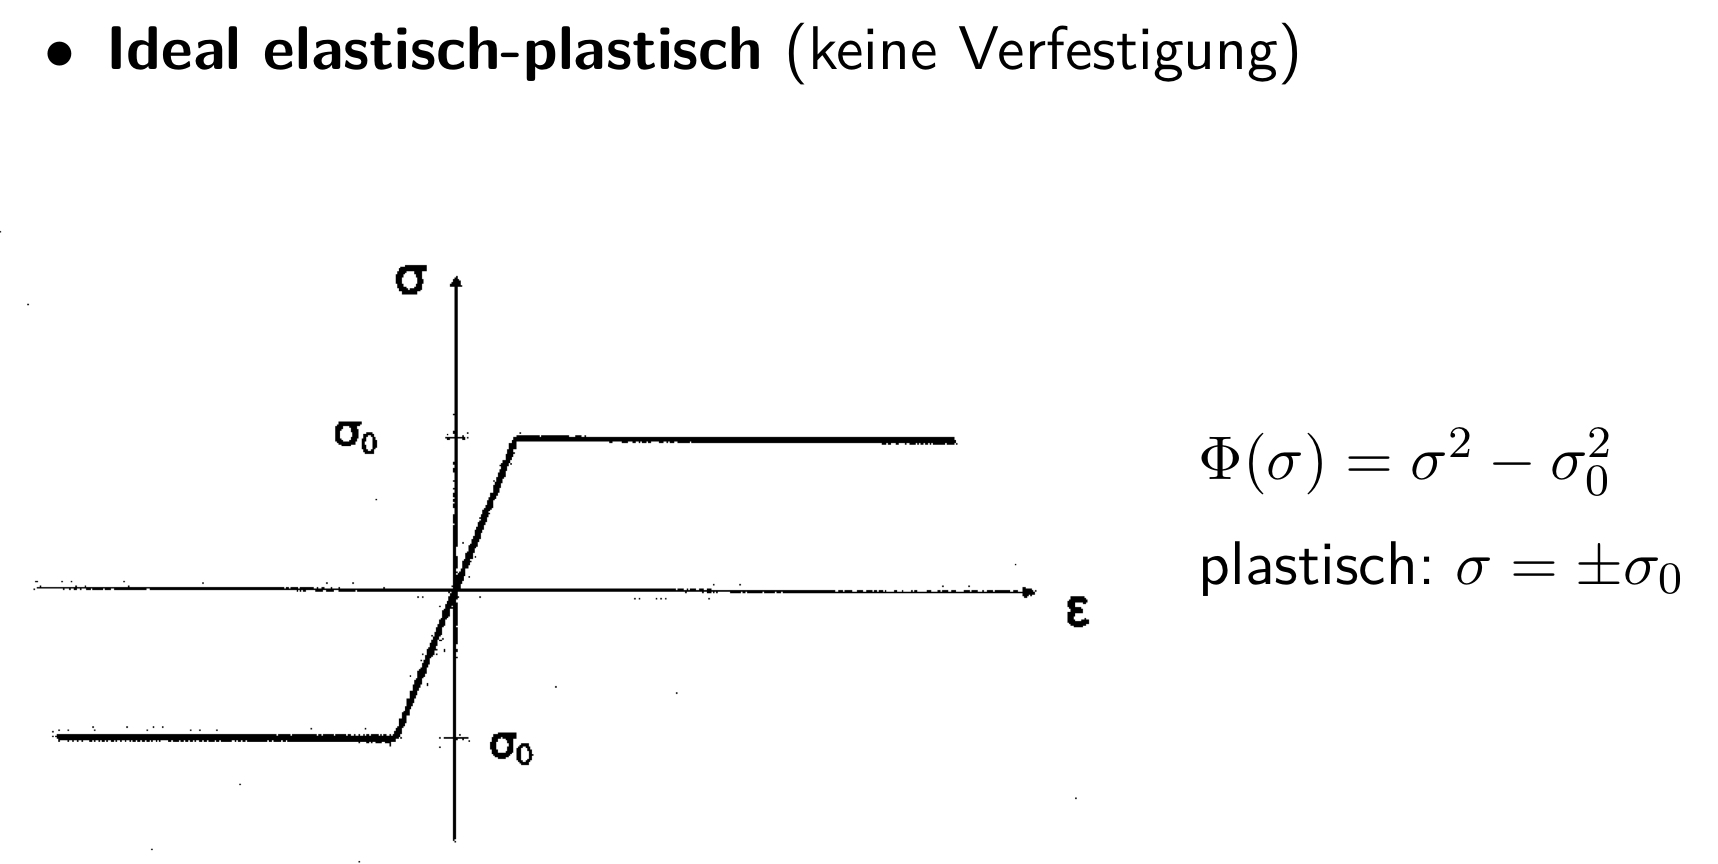
\includegraphics[width=0.5\linewidth]{04/Verf_ideal_elpl}
            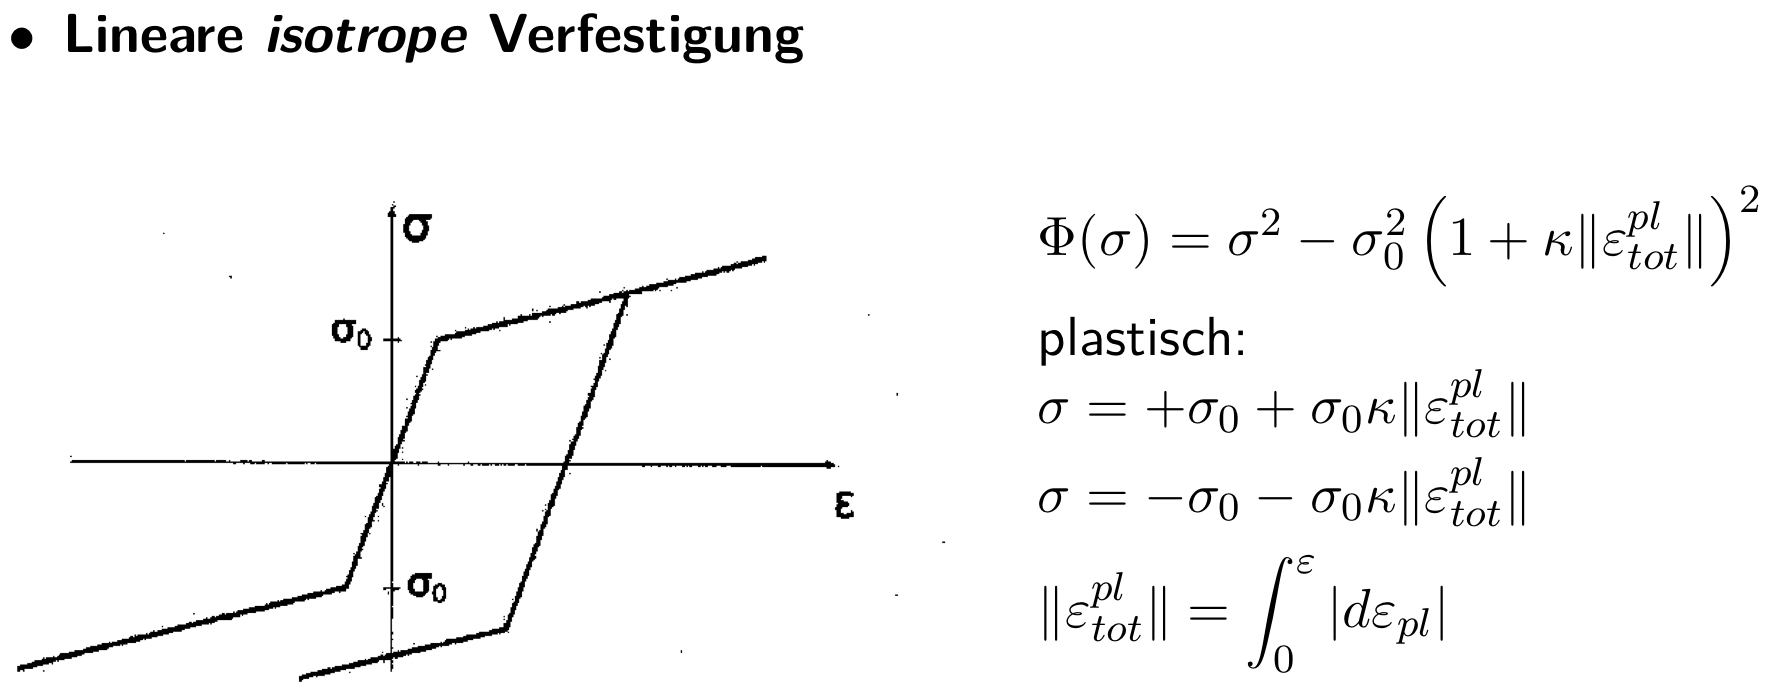
\includegraphics[width=0.5\linewidth]{04/Verf_lin_isotr}
            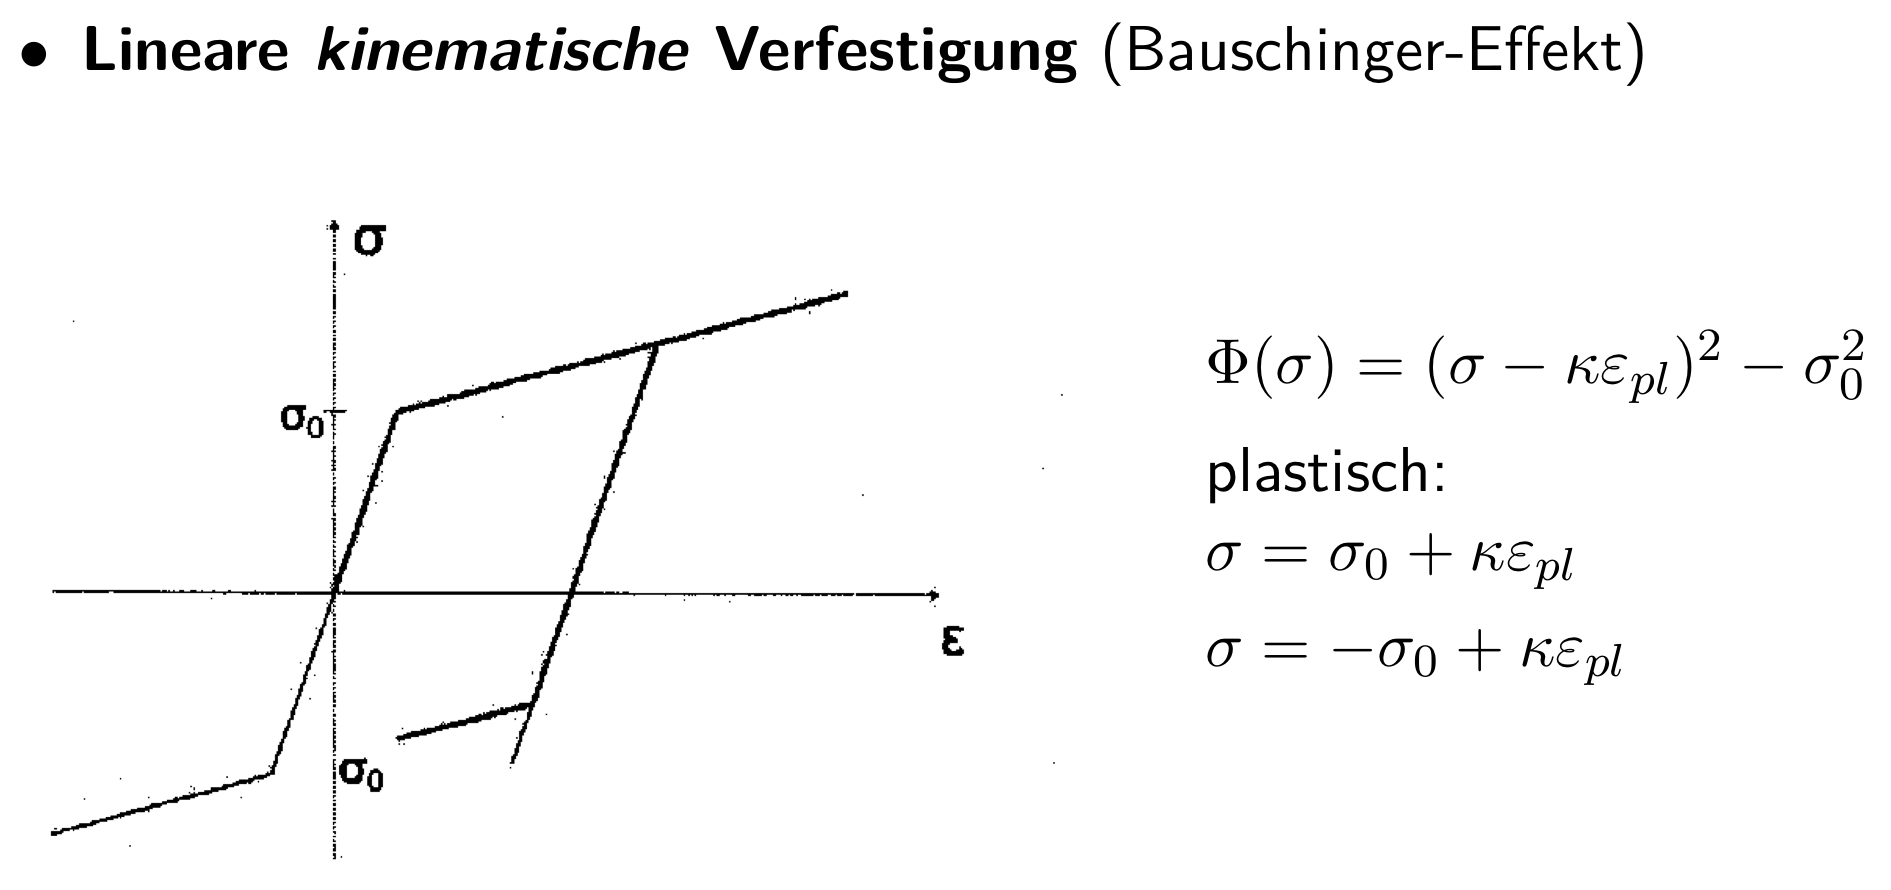
\includegraphics[width=0.5\linewidth]{04/Verf_lin_kin}
        \subsubsection{von Mieses'sche Vergleichsspannung}
            \vspace{-3mm}
            \[\Phi_{\textrm{v.Mises}}= \sigma_1^2+\sigma_2^2+\sigma_3^2-\sigma_1\sigma_2-\sigma_1\sigma_3-\sigma_2\sigma_3 -\sigma_0^2\quad(=0)\]
            \[\Leftrightarrow \sigma_{\textrm{v. Mises}}^{vgl}= \sqrt{\sigma_1^2+\sigma_2^2+\sigma_3^2-\sigma_1\sigma_2-\sigma_1\sigma_3-\sigma_2\sigma_3} \quad\textrm(HS)\]
        \subsubsection{Tresca'sche Vergleichsspannung}
            \textbf{Konservativer als von Mises'sche Vergleichsspannung} (Grenzfläche von Sechseck schneller erreicht als von Ellipse).
            \[\sigma_{\textrm{Tresca}}^{vgl}=\frac{1}{2}\textrm{max} \left(|\sigma_1-\sigma_2|,|\sigma_2-\sigma_3|,|\sigma_3-\sigma_1| \right) =\tau_0=\frac{\sigma_0}{2}\]
    \subsection{Statische Belastung}
        \begin{comment}
            \subsubsection{Kraft- \& Deformationsgesteurete Belastung:}
            $\frac{\varepsilon_b}{\varepsilon_0}$ Deformationsgesteurete Belastung. Bsp vorgespannte Schraube, therm Spannungen. Begrenzung weniger konservativ $\sigma\varepsilon$-Diagramm gr Dehnung führt zu nur kl Spannungserhöhung).\\ $\frac{\sigma_B}{\sigma_0}$ Kraftgesteuerte Belastung. (Für viele Metalle $\frac{\varepsilon_b}{\varepsilon_0} \gg \frac{\sigma_B}{\sigma_0}$) Überschreiten $R_{p0.2}$ weniger Reserve.
        \end{comment}
        \subsubsection{Spannungsverteilung}
            Falls homogen: bei Fliessgrenze wird die ganze Struktur plastifiziert. $\rightarrow$ Versagen %bei Erreichen der Fliessgrenze wird es in der ganzen Struktur zur Plastifizierung kommen. 
              
            Falls linear: es kommt an lokalen Stellen zu Plastifizierungen $\rightarrow$ Versagen erst bei einer grösseren Belastung.\\
            \textbf{Zug:}
            \begin{itemize}
                \item Erste plastifizierung = vollständige Plastifizierung:
            \end{itemize}
            \[F_{plast} = \sigma_0\ \cdot A\]
            
            %\columnbreak
            \textbf{Biegung:}
            \begin{itemize}
                \item Erste Plastifizierung:
            \end{itemize}
            \[M_{plast} = \sigma_0\cdot I\cdot\frac{1}{y_{\textrm{max}}} \quad\textrm{(mit bspw $\sigma_0 = R_p$)}\]
            \begin{itemize}
                \item Vollständige Plastifizierung:
            \end{itemize}
            \[M_{versagen} = 2\int_{-b/2}^{b/2}\int_{0}^{h/2}\sigma(y)ydydz \quad\textrm{mit $\sigma(y) = \sigma_0$}\]
            
        \columnbreak
        \subsubsection{Formfaktoren}
            Zug(homogen): $\frac{F_{versagen}}{F_{plast}}$\\
            Biegung(linear): $\frac{P_{versagen}}{P_{plast}}$ (Reserve, da Plastifizierung linear)
    \section{Kesselgleichungen}
        Für dünnwandige Behälter ($\frac{d}{R} \ll 1$)
        \vspace{-3mm}
        \[\sigma_{\varphi\varphi} = \frac{R}{d}P = 2\sigma_{zz}; \quad \sigma_{zz} = \frac{R}{2d}P; \quad \sigma_{rr}=0\]
            